%% Figure 1: Network Dimension Hierarchy
%% Auto-generated - Do not edit manually
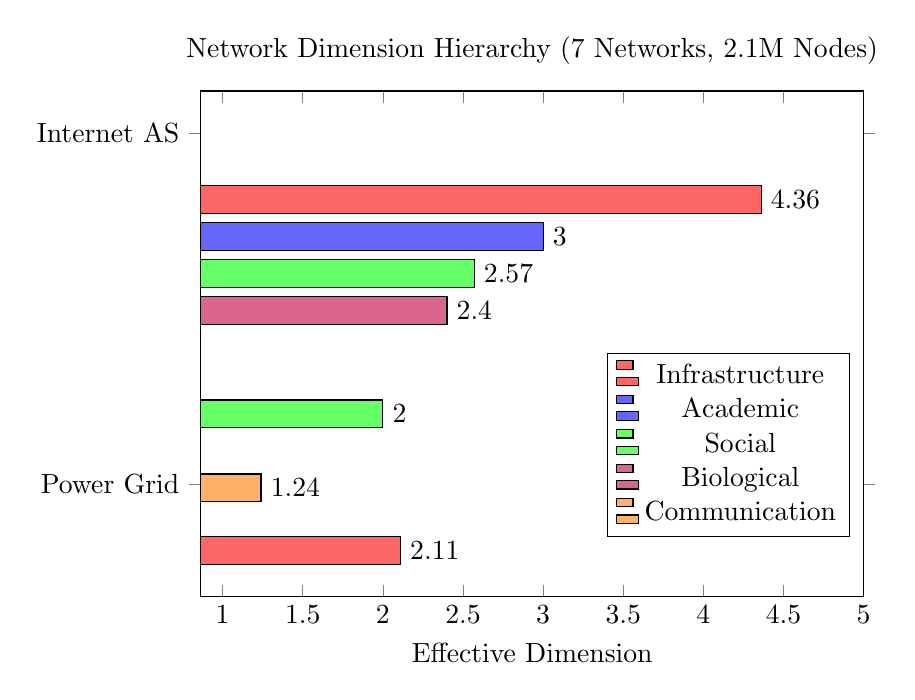
\begin{tikzpicture}
\begin{axis}[
    xbar,
    width=10cm,
    height=8cm,
    xlabel={Effective Dimension},
    title={Network Dimension Hierarchy (7 Networks, 2.1M Nodes)},
    symbolic y coords={Email, Power Grid, Twitter, Yeast PPI, Facebook, DBLP, Internet AS},
    ytick=data,
    nodes near coords,
    nodes near coords align={horizontal},
    enlarge y limits=0.1,
    xmax=5,
    legend style={at={(0.98,0.3)},anchor=east},
]
\addplot[fill=red!60] coordinates {(4.36,Internet AS) (2.11,Power Grid)};
\addplot[fill=blue!60] coordinates {(3.0,DBLP)};
\addplot[fill=green!60] coordinates {(2.57,Facebook) (2.0,Twitter)};
\addplot[fill=purple!60] coordinates {(2.4,Yeast PPI)};
\addplot[fill=orange!60] coordinates {(1.24,Email)};
\legend{Infrastructure, Academic, Social, Biological, Communication}
\end{axis}
\end{tikzpicture}
